\documentclass[11pt,green,twocol,citestyle=authoryear, bibstyle=authoryear]{elegantbook}

%\documentclass[pad]{elegantbook}

\title{Academic Notes Series: No. 1}
\subtitle{Financial Decisions and Markets: A Course for Asset Pricing}

\author{Hang Cheng}
\institute{School of Finthch \& DUFE}
\date{\today}
\version{0.1}
\bioinfo{Website}{chenghang.work}

\extrainfo{Work Hard, Study Hard.}

\logo{LOGO.png}
\cover{cover.jpg}

% modify the color in the middle of titlepage
\definecolor{customcolor}{RGB}{32,178,170}
\colorlet{coverlinecolor}{customcolor}
\usepackage{cprotect}

\addbibresource[location=local]{reference.bib} % bib


\begin{document}

\maketitle

\frontmatter
\tableofcontents

\mainmatter
\chapter*{Introduction}
\markboth{Introduction}{Introduction}
This is academic note for \cite{Campbell_2017} and this project is beginning from September 10, 2022.


\chapter{Choice under Uncertainty}

\begin{introduction}
\item Expected Utility 
\end{introduction}

This chapter review the basic theory of choice under Uncertainty, ignoring time by assuming that all Uncertainty is resolved at a single future data. 

Related Literature:

\begin{itemize}
    \item \cite{Gollier_2001}
    \item \cite{Ingersoll_1987}
\end{itemize}

\section{Expected Utility}

\begin{proposition}
    \begin{itemize}
        \item An ordinal utility function $ \Upsilon(.) $ tells you that an agent is indifferent between $ x $ and $ y $ if $ \Upsilon(x)=\Upsilon(y) $  and prefers $ x $ to $ y $ if $ \Upsilon(x)>\Upsilon(y) $.   
        \item For any strictly increasing function $ \Theta $, the preferences expressed by $ \Theta(\Upsilon(.)) $ are the same as those expressed by $ \Upsilon $. 
    \end{itemize}
\end{proposition}

\chapter{Static Portfolio Choice}

\chapter{Static Equilibrium Asset Pricing}

\begin{introduction}
    \item CAPM
\end{introduction}

\section{The Capital Asset Pricing Model (CAPM)}

Some basic assumption:
\begin{itemize}
    \item All investors are price-takers
    \item Evaluate portfolios using the means and variances of single-period returns
    \item Investors have common beliefs about the means, variances, and covariances of returns.
    \item There are no nontraded assets, taxes, or transactions costs.
    \item Investors can borrow or lend at a given riskfree interest rate.
\end{itemize}

\begin{note}
    The market portfolio is mean-variance efficient.
\end{note}

\subsection{Asset Pricing Implication of the Sharpe-Lintner CAPM}

An increase in the weight of asset $ i $ in portfolio $ p $, $ \omega_i $, financed by a decrease in the weight on the riskless asset, affect the mean and variance of the return on portfolio $ p $ as follows:
\begin{equation}\label{equ:3.1}
    \begin{aligned}
        &\overline{R}_p=\sum_i w_i\left(\overline{R_{i}}-R_f\right) \\
        &\frac{d R_p }{d w_i}=\overline{R_i}-R_f
        \end{aligned}
\end{equation}  

\begin{equation}\label{equ:3.2}
    \frac{d \operatorname{Var}\left(R_p\right)}{d w_i}=2 \operatorname{Cov}\left(R_i, R_p\right)
\end{equation} 

\begin{proof}
    The individual-asset variance and covariances in $ Var(R_p) $ are
\begin{equation*}
    Var(R_p)= 2 w_i w_1 \operatorname{Cov}\left(R_i, R_1\right)+\cdots+w_i^2 \operatorname{Var}\left(R_i\right)+\cdots+2 w_i w_N \operatorname{Cov}\left(R_i, R_N\right) 
\end{equation*} 
\begin{equation}\label{equ:3.3}
       \frac{d \operatorname{Var}\left(R_p\right)}{d w_i} = 2 w_1 \operatorname{Cov}\left(R_i, R_1\right)+\cdots+2 w_i \operatorname{Var}\left(R_i\right) +\cdots+2 w_N \operatorname{Cov}\left(R_i, R_N\right)=2 \operatorname{Cov}\left(R_i, R_p\right)
\end{equation}
\end{proof}

The ratio of the effect on mean, (\ref{equ:3.1}), to the effect on variance, (\ref{equ:3.2}) in
\begin{equation}\label{equ:3.4}
    \frac{d \bar{R}_p / d w_i}{d \operatorname{Var}\left(R_p\right) / d w_i}=\frac{\bar{R}_i-R_f}{2 \operatorname{Cov}\left(R_i, R_p\right)}
\end{equation}

\begin{proposition}
    If portfolio $ p $  is mean-variance efficient, this ratio should be the same for all individual assets $ i $.
\end{proposition}
\begin{proof}
    \begin{equation}\label{equ:3.5}
        d \bar{R}_p=\left(\bar{R}_i-R_f\right) d w_i+\left(\bar{R}_j-R_f\right) d w_j
    \end{equation}
    and
    \begin{equation}\label{equ:3.6}
        d \operatorname{Var}\left(R_p\right)=2 \operatorname{Cov}\left(R_i, R_p\right) d w_i+2 \operatorname{Cov}\left(R_j, R_p\right) d w_j
    \end{equation}
    Now consider setting $ dw_j $ so that the mean portfolio return is unchanged, $ d\overline{R_p} = 0 $:
    \begin{equation}\label{equ:3.7}
        d w_j=-\frac{\left(\bar{R}_i-R_f\right)}{\left(\bar{R}_j-R_f\right)} d w_i
    \end{equation}  
    The portfolio variance must also be unchanged. We have
    \begin{equation}\label{equ:3.8}
        d \operatorname{Var}\left(R_p\right)=\left[2 \operatorname{Cov}\left(R_i, R_p\right)-2 \operatorname{Cov}\left(R_j, R_p\right) \frac{\left(\bar{R}_i-R_f\right)}{\left(\bar{R}_j-R_f\right)}\right] d w_i=0
    \end{equation}
    This requires
    \begin{equation}\label{equ:3.9}
        \frac{\bar{R}_i-R_f}{2 \operatorname{Cov}\left(R_i, R_p\right)}=\frac{\bar{R}_j-R_f}{2 \operatorname{Cov}\left(R_j, R_p\right)}
    \end{equation}
    This equation must hold for all assets $ j $, including the original portfolio itself. Setting
    $ j = p $, we get
    \begin{equation}\label{equ:3.10}
        \frac{\bar{R}_i-R_f}{2 \operatorname{Cov}\left(R_i, R_p\right)}=\frac{\bar{R}_p-R_f}{2 \operatorname{Var}\left(R_p\right)}
    \end{equation}
    or
    \begin{equation}\label{equ:3.11}
        \bar{R}_i-R_f=\frac{\operatorname{Cov}\left(R_i, R_p\right)}{\operatorname{Var}\left(R_p\right)}\left(\bar{R}_p-R_f\right)=\beta_{i p}\left(\bar{R}_p-R_f\right)
    \end{equation}
    where $ \beta_{i p} \equiv \operatorname{Cov}\left(R_i, R_p\right) / \operatorname{Var}\left(R_p\right) $ is the regression coefficient of asset $ i $'s return on portfolio $ p $'s return.
\end{proof}

The market portfolio $ m $ is mean-variance efficient. Under the restriction (\ref{equ:3.11}) describes the market portfolio:
\begin{equation}\label{equ:3.12}
    \bar{R}_i-R_f=\beta_{i m}\left(\bar{R}_m-R_f\right)
\end{equation}
The regression of excess return on the market excess return,
\begin{equation}\label{equ:3.13}
    R_{i t}-R_{f t}=\alpha_i+\beta_{i m}\left(R_{m t}-R_{f t}\right)+\epsilon_{i t}
\end{equation}
the intercept $ \alpha_i $ should be $ 0 $ for all assets. $ \alpha_i $ is called \textit{Jensen's alpha}.

\subsection{The Black CAPM}
\begin{figure}[!h]
    \centering
    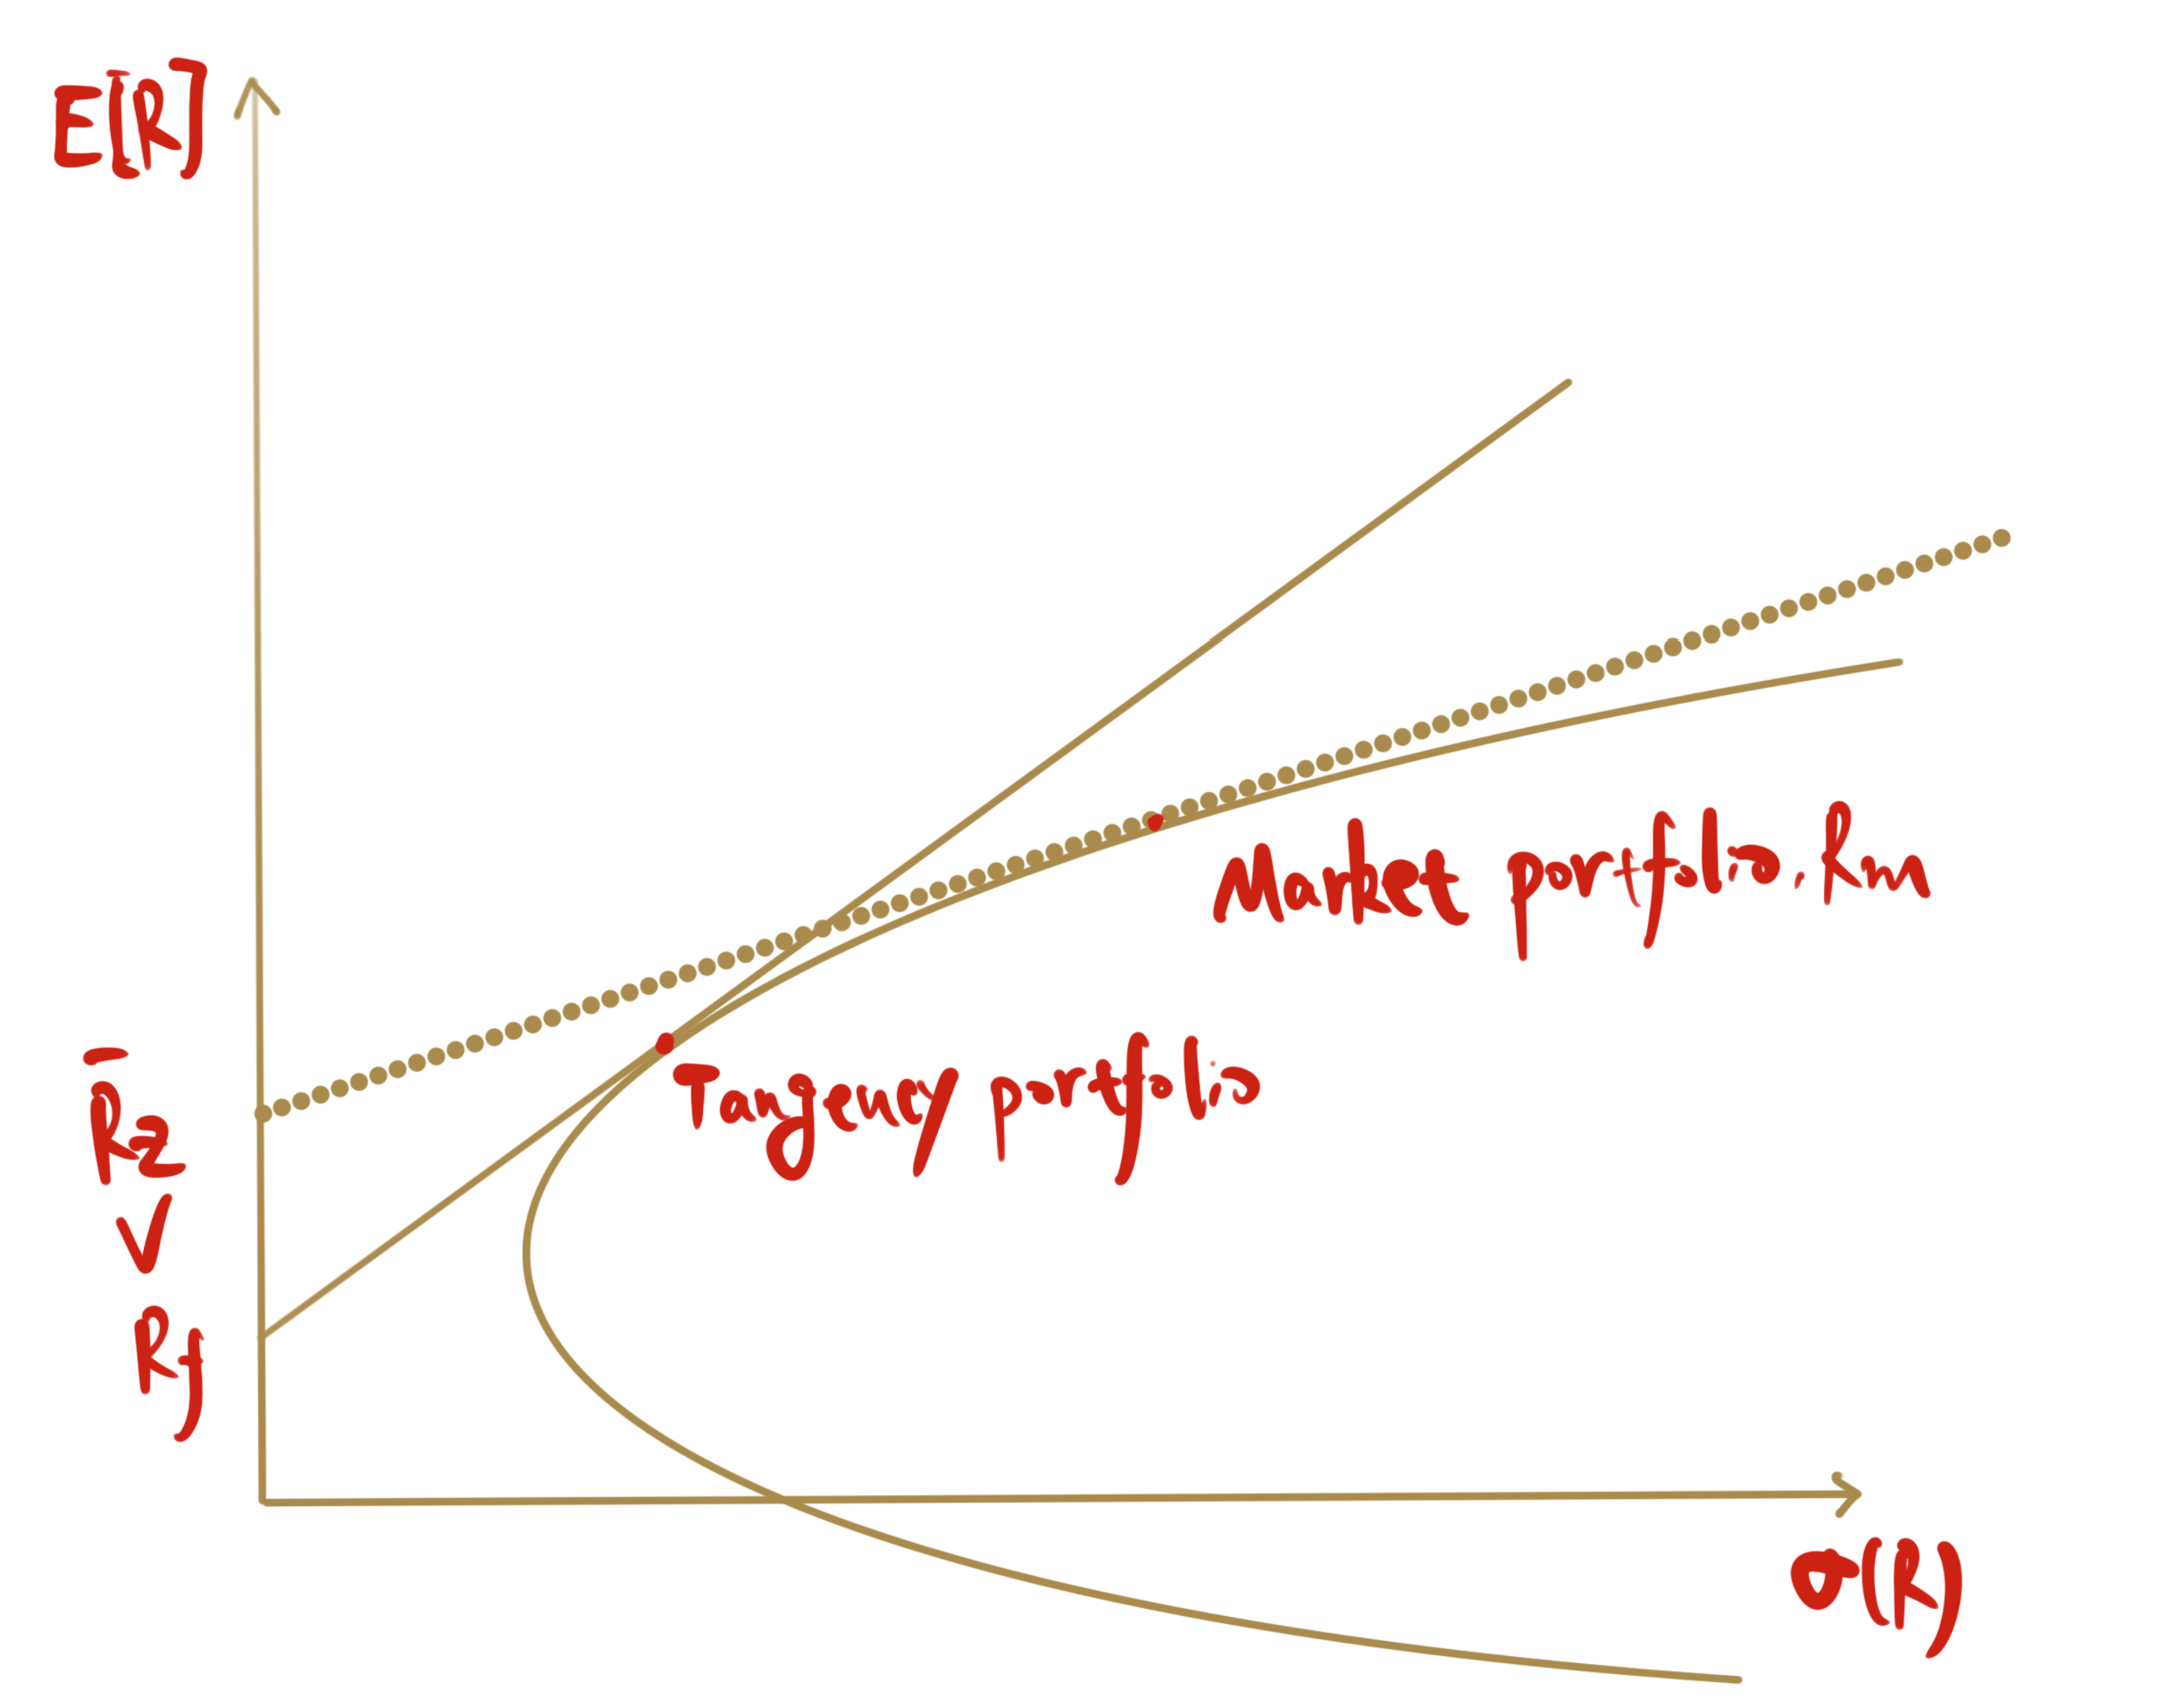
\includegraphics[width = 0.6\textwidth]{blackcapm.pdf}
    \caption{The Black (1972) CAPM}
\end{figure}

\subsection{Beta Pricing and Portfolio Choice}

\begin{problem}
    Assume that the Sharpe-Lintner CAPM holds, so the mean-variance efficient frontier consists of combinations of Treasury bills and the market portfolio. Nonetheless, some households make the mistake of holding undiversified portfolios that contain only one stock or a few stocks. (Empirical evidence on such behavior is discussed in Chapter 10.)
    \begin{enumerate}
        \item Show that the Sharpe ratio of any portfolio divided by the Sharpe ratio of the market
        portfolio equals the correlation of that portfolio with the market portfolio.
        \item Suppose the market is made up of identical stocks, each of which has the same market capitalization, the same mean and variance of return, and the same correlation $ \rho > 0 $, with every other individual stock. Consider the limit as the number of stocks
        in the market increases. What is the Sharpe ratio of an equally-weighted portfolio
        that contains N stocks divided by the Sharpe ratio of the market portfolio? Interpret.
    \end{enumerate}
\end{problem}

\begin{solution}
\begin{enumerate}
    \item The Sharpe ratio of portfolio $ p $ divided by the Sharpe ratio of the market portfolio equals to
    \begin{equation*}
        \begin{aligned}
            &\frac{E\left(R_p-R_f\right)}{\sigma\left(R_p\right)} / \frac{E\left(R_m-R_f\right)}{\sigma\left(R_m\right)} \\
            &=\frac{\beta_{p m} E\left(R_m-R_f\right)}{\sigma\left(R_p\right)} / \frac{E\left(R_m-R_f\right)}{\sigma\left(R_m\right)} \\
            &=\frac{\beta_{p m} \sigma\left(R_m\right)}{\sigma\left(R_p\right)} \\
            &=\frac{\operatorname{cov}\left(R_p \cdot R_m\right) \cdot \sigma\left(R_m\right)}{\operatorname{Var}\left(R_m\right) \cdot \sigma\left(R_p\right)} \\
            &=\frac{\rho \sigma\left(R_p\right) \sigma\left(R_m\right) \cdot \sigma\left(R_m\right)}{\operatorname{Var}\left(R_m\right) \cdot \sigma\left(R_p\right)}\\
            &=\rho
        \end{aligned}
    \end{equation*}
    where $ \rho $ is the correlation coefficient between portfolio $ r_p $ and $ r_m $.   
    \item The equal-weighted portfolio $ p $  contains $ N $ stocks. So the return and variance of this portfolio is 
    \begin{equation*}
        r_p=\frac{1}{N} r_1+\frac{1}{N} r_2+\ldots+\frac{1}{N} r_N=r
    \end{equation*}  
    \begin{equation*}
        \begin{aligned}
            &\begin{aligned}
            &\sigma_p^2=\frac{1}{N^2} \sigma^2\left(r_1\right)+\frac{1}{N^2}\sigma^2\left(r_1\right)+\cdots \\
            & + 2\frac{1}{N^2} \operatorname{cov}\left(r_1, r_2\right)+\cdots+2 \frac{1}{N^2} \operatorname{cov}\left(r_{N-1}, r_N\right)
            \end{aligned}\\
            &=\frac{1}{N} \sigma^2+\frac{2}{N^2} \cdot \frac{N-1}{2} \cdot N \cdot \rho \sigma^2\\
            &=\frac{1}{N} \sigma^2+\frac{N-1}{N} \rho \sigma^2\\
            &=\rho \sigma^2+\frac{1}{N} \sigma^2(1-\rho)
            \end{aligned}
    \end{equation*}
    when $ N\rightarrow \infty  $, the variance of market portfolio is 
    \begin{equation*}
        \sigma ^2_{m} = \rho \sigma^2
    \end{equation*} 
    The Sharpe ratio's ratio is 
    \begin{equation*}
        \begin{aligned}
            &\frac{\sqrt{\rho \sigma^2}}{\sqrt{\rho \sigma^2+\frac{1}{N} \sigma^2(1-\rho)}} \\
            &=\sqrt{\frac{N \rho}{N \rho +1-\rho}}
            \end{aligned}
    \end{equation*}
\end{enumerate}
\end{solution}

\section{Arbitrage Pricing and Multifactor Models}

\subsection{Arbitrage Pricing in a Single-Factor Model}

\begin{equation*}
    \begin{aligned}
        R_{i t}^e = \alpha_i+\beta_{i m} R_{m t}^e+\epsilon_{i t} \\
        \mathrm{E}\left[\epsilon_{i t} \epsilon_{j t}\right]=0 \\
        \operatorname{Cov}\left(R_{i t}^e, R_{j t}^e\right)=\beta_{i m} \beta_{j m} \sigma_m^2
    \end{aligned}
\end{equation*}
The implication of above assumption is that:

\begin{remark}
    If many assets are available, we should expect $ \alpha_i $ typically to be very small in absolute value. This is the \textit{arbitrage pricing theory} of \cite{Ross_1976}.
\end{remark}

\textbf{Why?}

Portfolio of $ N $ assets $ i $, the excess return on the portfolio will be
\begin{equation*}
    R_{p t}^e=\alpha_p+\beta_{p m} R_{m t}^e+\epsilon_{p t}
\end{equation*}  
where $ \alpha_p=\sum_{j=1}^N w_j \alpha_j, \beta_{p m}=\sum_{j=1}^N w_j \beta_{j m}, \text { and } \epsilon_{p t}=\sum_{j=1}^N w_j \epsilon_{j t} $. 

The variance of $ \epsilon_{p t} $ will be 
\begin{equation*}
    \operatorname{Var}\left(\epsilon_{p t}\right)=\sum_{j=1}^N w_j^2 \operatorname{Var}\left(\epsilon_{j t}\right)
\end{equation*}
which will shrink rapidly with $ N $  provided that no single weight $ w_j $  is too large.

Suppose that the portfolio has enough stocks, with a small enough weight in each one, that the residual risk $ \operatorname{Var}\left(\epsilon_{p t}\right) $ is negligible. We say that the portfolio is \textbf{well diversified}. For such a portfolio, we can neglect $ \epsilon_{p t} $ and write the excess return as
\begin{equation*}
    R_{p t}^e=\alpha_p+\beta_{p m} R_{m t}^e
\end{equation*}
But we must have $ \alpha_p  = 0 $. If not, there is an arbitrage opportunity: go short $ \beta_{pm} $ units of the market and go long on unit of portfolio $ p $, while funding all positions with riskless borrowing and lending. This delivers a riskless excess return of $ \alpha_p $.  

\cite{Ross_1976} exploits this insight, showing that $ \alpha_p = 0 $ for all well-diversified portfolios implies that ``almost all'' individual assets have $ \alpha_i $ very close to zero. Technically, the result is that if idiosyncratic variance of individual assets are bounded above, then
\begin{equation*}
    \lim _{N \rightarrow \infty} \frac{1}{N} \sum_{i=1}^N \alpha_i^2=0
\end{equation*}
\begin{proof}
    Consider forming an alpha-weighted portfolio by making dollar investment (this is the weight) of 
    \begin{equation*}
        \frac{\alpha_i}{\sqrt{N \sum_{i=1}^N \alpha_i^2}}
    \end{equation*}
    So the payoff on this portfolios is 
    \begin{equation*}
        \frac{\sum_{i=1}^N \alpha_i R_{i t}}{\sqrt{N \sum_{i=1}^N \alpha_i^2}}=\frac{\sum_{i=1}^N \alpha_i\left(R_{f t}+\alpha_i+\beta_{i m} R_{m t}^e+\epsilon_{i t}\right)}{\sqrt{N \sum_{i=1}^N \alpha_i^2}}
    \end{equation*}
    We make two additional assumption: 
    \begin{enumerate}
        \item \begin{equation*}
            \lim _{N \rightarrow \infty} \frac{\sum_{i=1}^N \alpha_i}{\sqrt{N \sum_{i=1}^N \alpha_i^2}}=0
        \end{equation*}
        \item \begin{equation*}
            \lim _{N \rightarrow \infty} \frac{\sum_{i=1}^N \alpha_i \beta_{i m}}{\sqrt{N \sum_{i=1}^N \alpha_i^2}}=0
        \end{equation*}
    \end{enumerate}
    In other words, that as the number of assets increase ($ N \rightarrow \infty  $), the total initial dollar investment is zero, and the portfolio has a zero beta with market.

    So the limiting payoff on the alpha-weighted portfolio has only 2 components:
    \begin{equation}\label{equ:alpha-weighted portfolio}
        \lim _{N \rightarrow \infty} \frac{\sum_{i=1}^N \alpha_i R_{i t}}{\sqrt{N \sum_{i=1}^N \alpha_i^2}}=\sqrt{\frac{\sum_{i=1}^N \alpha_i^2}{N}}+\frac{\sum_{i=1}^N \alpha_i \epsilon_{i t}}{\sqrt{N \sum_{i=1}^N \alpha_i^2}}
    \end{equation}
    The variance of the payoff in equation (\ref{equ:alpha-weighted portfolio}) is 
    \begin{equation*}
        \frac{\operatorname{Var}\left(\sum_{i=1}^N \alpha_i \epsilon_{i t}\right)}{N \sum_{i=1}^N \alpha_i^2}=\frac{\sum_{i=1}^N \alpha_i^2 \sigma_i^2}{N \sum_{i=1}^N \alpha_i^2} = 0
    \end{equation*}
    So the first term of equation (\ref{equ:alpha-weighted portfolio}) should equal to zero, which is 
    \begin{equation*}
        \lim _{N \rightarrow \infty} \frac{1}{N} \sum_{i=1}^N \alpha_i^2=0 
    \end{equation*}
\end{proof}

\subsection{Multifactor Models}

\section{Empirical Evidence}

\subsection{Test Methodology}

\subsubsection{Time-Series Approach}
\begin{equation}\label{equ:capm-ts}
    R_{i t}-R_{f t}=\alpha_i+\beta_{i m} (R_{m t}-R_{f t})+\epsilon_{i t}
\end{equation}
The null hypothesis is that $ \alpha = 0 $. 
\begin{note}
    The challenge is to test it jointly for a set of $ N $ assets.
\end{note}

\subsubsection{Cross-Section Approach}

\subsubsection{Fama-MacBeth Approach}

\subsection{The CAPM and the Cross-Section of Stock Returns}
\begin{itemize}
    \item $ \mathbf{\beta} $
    \item \textbf{Size}  
    \item \textbf{Value}
    \item \textbf{Momentum}
    \item \textbf{Post-event drift}
    \item \textbf{Turnover and volatility}
    \item \textbf{Insider trading}
    \item \textbf{Growth of the firm}. Total asset growth
    \item \textbf{Earning quality}
    \item \textbf{Profitability}
\end{itemize}

\chapter{The Stochastic Discount Factor}


\printbibliography[heading=bibintoc, title=\ebibname]


\appendix


\chapter{Nothing}




\end{document}